\documentclass[tikz,convert={outfile=\jobname.svg}]{standalone}
\usepackage{tikz}
\usetikzlibrary{automata, positioning, arrows.meta, bending} % 'positioning' is helpful for arranging nodes

\begin{document}
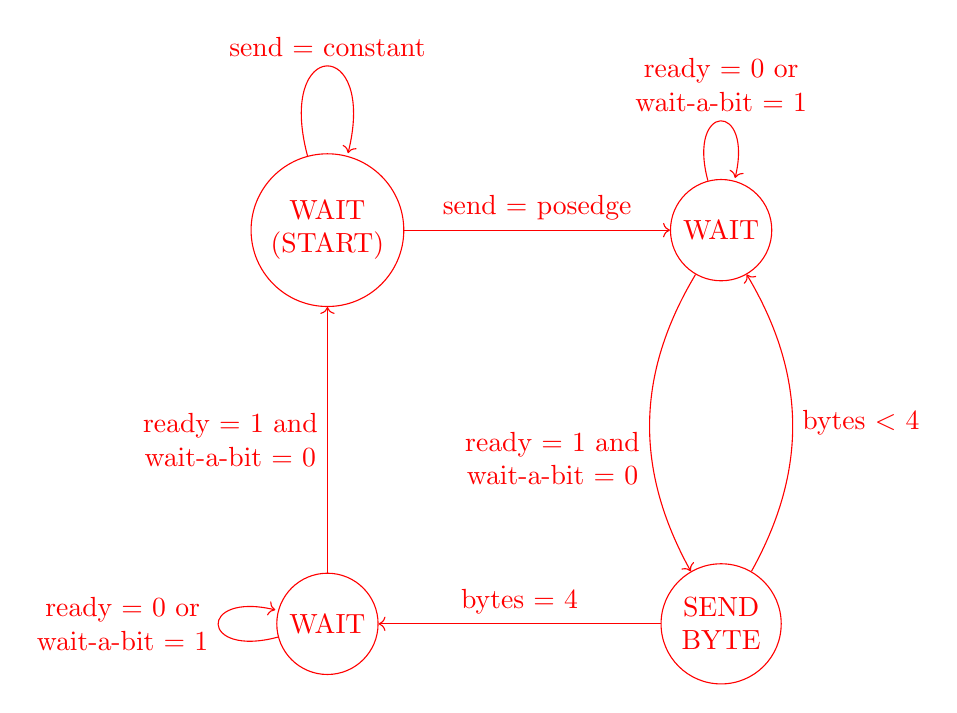
\begin{tikzpicture}[node distance=5cm, auto, state/.style={draw=red,shape=circle,text=red}, every node/.style={text=red}]

    % Define the states (nodes)
    \node[state, align=center] (s0) {WAIT\\(START)}; % Initial state 'q0'
    \node[state, right of=s0] (s2) {WAIT};
    \node[state, below of=s2,align=center] (s1) {SEND\\BYTE}; % Accepting state 'q1', positioned to the right of 'q0'
    \node[state, below of=s0] (s3){WAIT};
    % Define the transitions (edges)
    \path[->, draw=red] %[draw = red]
    (s0) edge node[above] {send = posedge} (s2) % Transition from q0 to q1 labeled 'a'
    (s1) edge node[above] {bytes = 4} (s3) % Transition from q0 to q1 labeled 'a'
    (s0) edge [loop above] node {send = constant} (s0) % Transition from q1 to q0 labeled 'b'
    (s1) edge[bend right] node[right] {bytes $<$ 4} (s2)
    (s2) edge [bend right] node[below left,align=center] {ready = 1 and\\wait-a-bit = 0} (s1)
    (s2) edge [loop above] node[align=center] {ready = 0 or\\wait-a-bit = 1} (s2)
    (s3) edge[loop left] node[left, align=center]{ready = 0 or\\wait-a-bit = 1} (s3)
    (s3) edge node[left, align=center]{ready = 1 and\\wait-a-bit = 0} (s0);
\end{tikzpicture}
\end{document}

